\documentclass[journal]{IEEEtran}
%
\usepackage{instructivo}  
\graphicspath{{./}{./fig/}}

\usepackage{circuitikz}
\usepackage{float}
\usepackage{graphicx}
\usepackage[skip=5pt]{caption}
\usepackage{flafter}
\usepackage{needspace}
\usepackage{csquotes}
\usepackage{upgreek}


\hyphenation{op-tical net-works semi-conduc-tor}

\renewcommand\IEEEkeywordsname{Palabras clave}

\begin{document}
\title{Topologías de amplificadores de fuente común y de drenador común con JFETs}


\author{Juan~P.~Elizondo~Espinoza,~\IEEEmembership{Estudiante,~TEC}
        y~Matías~A.~Camacho~Abarca,~\IEEEmembership{Estudiante,~TEC.}
}


\markboth{TEC.~EL-3215 Laboratorio de Electrónica Analógica, IS~2025}%
{EL3215 Laboratorio de Electrónica Analógica}


\maketitle


\begin{abstract}
El objetivo del experimento fue construir circuitos recortadores para entender el comportamiento de la onda de salida
teniendo en cuenta distintos casos de polarización. Se logró comprobar el comportamiento teórico esperado de los circuitos a través de un análisis visual.
\end{abstract}

\begin{IEEEkeywords}
Diodo, tensión, corriente, junta, ruptura.
\end{IEEEkeywords}


%%%%%%%%%%%%%%%%%%%%%%%%%%%%%%%%%%%%%%%%%%%%%%%%%%%%%%%%%%%%%%%%%%%%%%%%%%%%%%%%%%%%%%%%%%%%%%
%%%%%%%%%%%%%%%%%%%%%%%%%%%%%%%%%%%%%%%%%%%%%%%%%%%%%%%%%%%%%%%%%%%%%%%%%%%%%%%%%%%%%%%%%%%%%%
\section{Introducción}

\IEEEPARstart{U}n diodo es un componente electrónico de dos terminales que permite el flujo de corriente en una dirección y lo bloquea en la otra. Está formado por la unión de dos materiales semiconductores con diferente tipo de dopaje: tipo p y tipo n.

El material tipo p se forma al dopar semiconductores como el silicio o el germanio con impurezas de tres electrones de valencia, como el boro, lo que genera una abundancia de huecos (cargas positivas). Por otro lado, el material tipo n se obtiene al agregar impurezas con cinco electrones de valencia, como el fósforo o el arsénico, lo que introduce electrones libres en la estructura.

Al unir ambos materiales en un solo dispositivo, se forma una unión pn, la base del funcionamiento del diodo. Idealmente, los huecos pueden moverse desde la región p hacia la región n, siguiendo la dirección de la corriente convencional. Sin embargo, si se intenta conducir corriente en la dirección opuesta (de n a p), la unión pn presenta una barrera que impide el flujo, actuando como un interruptor unidireccional.

Estas propiedades aplican para diodos ideales, ya que en la realidad los diodos tienen un rango de tensión necesario para que la
corriente fluya significativamente en polarización directa (corriente convencional de p a n). Los diodos incluso tienen corriente en polarización inversa (corriente convencional de n a p), aunque esta suele ser despreciable. Sin embargo, para efectos de análisis, se pueden 
generalizar muchas de estas propiedades.

Uno de los usos más particulares de los diodos es en circuitos recortadores. Estos se aprovechan del funcionamiento del diodo como una fuente de tensión en polarización directa
y como un nodo abierto en inversa. En estas aplicaciones, se elimina partes de la señal de entrada por encima o por debajo de cierto nivel de voltaje. Existen dos configuraciones principales: en serie y en paralelo.  

En los recortadores en paralelo, el diodo se coloca en paralelo con la carga y conduce solo cuando la señal supera un voltaje específico. Si el diodo está sin polarización externa, su umbral de conducción es aproximadamente 0 V en el modelo ideal.   

Estos circuitos son útiles para limitar amplitudes y proteger componentes sensibles frente a sobrevoltajes. En el modelo ideal, el diodo cambia instantáneamente entre conducción y no conducción, lo que permite una representación simplificada del comportamiento del circuito. \cite{Boylestad}


%%%%%%%%%%%%%%%%%%%%%%%%%%%%%%%%%%%%%%%%%%%%%%%%%%%%%%%%%%%%%%%%%%%%%%%%%%%%%%%%%%%%%%%%%%%%%%
%%%%%%%%%%%%%%%%%%%%%%%%%%%%%%%%%%%%%%%%%%%%%%%%%%%%%%%%%%%%%%%%%%%%%%%%%%%%%%%%%%%%%%%%%%%%%%
\section{Circuitos recortadores con Diodos}
Como una forma de entender el funcionamiento de estos dispositivos (los Diodos), se pueden diseñar circuitos que tengan amplias aplicaciones prácticas en la vida cotidiana,
dentro de estos están los circuitos recortadores, en donde los diodos juegan un papel muy importante y es posible establecer diferentes configuraciones según se requiera. 


\subsection{Circuitos de Medición}

\begin{figure}[H]
        \centering
        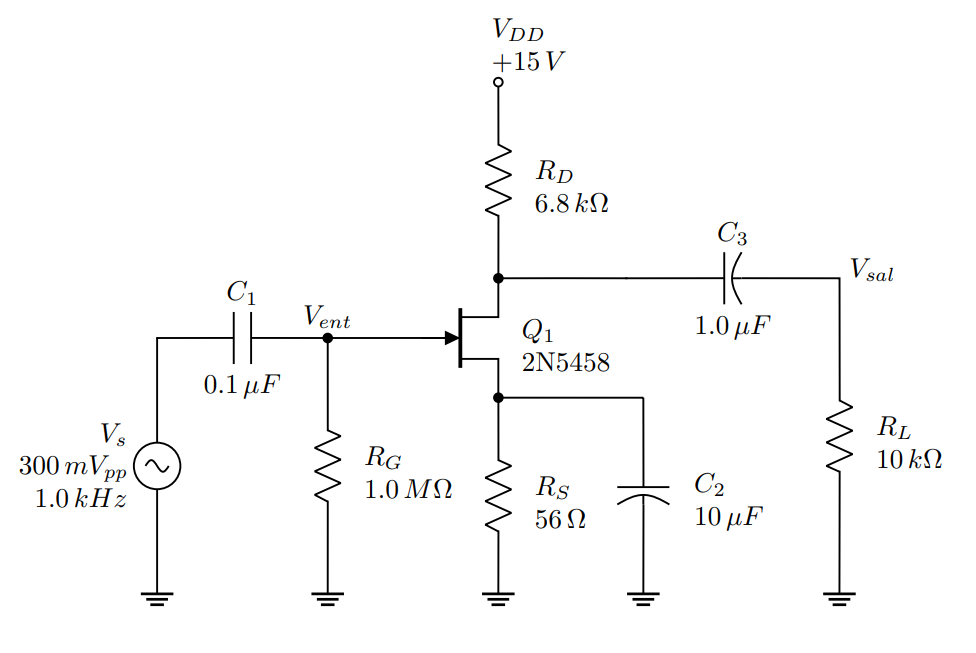
\includegraphics[width=3.4in]{Circ1.png}
        \caption{Circuito 1}
        \label{fig:Circuito1}
\end{figure}

\begin{figure}[H]
        \centering
        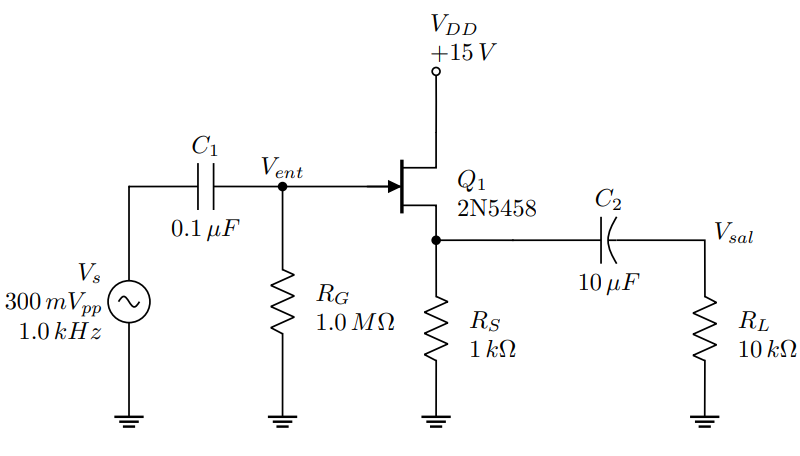
\includegraphics[width=3.4in]{CIRC2.png}
        \caption{Circuito 2}
        \label{fig:Circuito2}
\end{figure}

\begin{figure}[H]
        \centering
        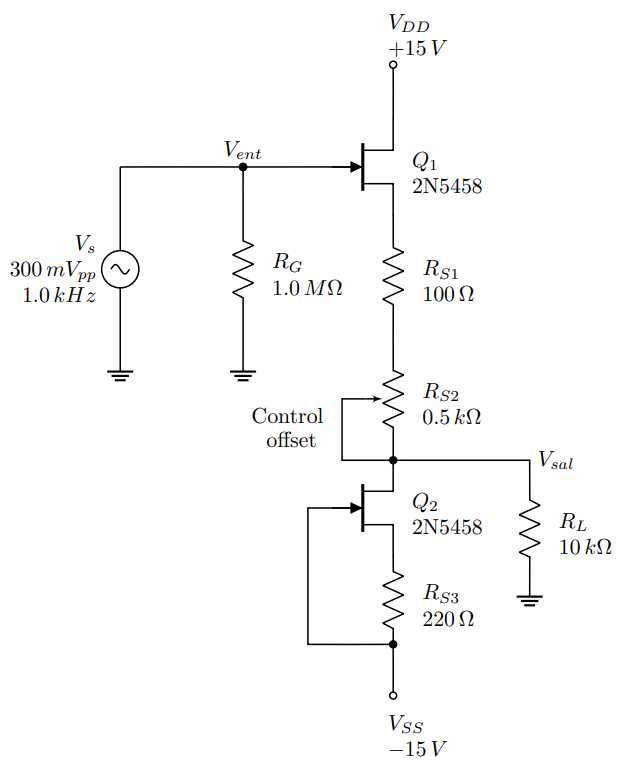
\includegraphics[width=3.4in]{CIRC2_2.png}
        \caption{Circuito 3}
        \label{fig:Circuito2_2}
\end{figure}

\needspace{5\baselineskip}


\subsection{Resultados}

\begin{table}[H]
        \centering
        \renewcommand{\arraystretch}{1.5}
        \caption{Valores de resistencias utilizadas en el circuito 1}
        \begin{tabular}{ >{\centering\arraybackslash}m{2.5cm} >{\centering\arraybackslash}m{2.5cm} >{\centering\arraybackslash}m{2.5cm} }
                \hline
            \centering
            Componente & Valor requerido & Valor medido\\ 
            \hline
            \centering
            $R_G$ & $1$ $\mathrm{M}\Omega$ & $1.014~22$ $\mathrm{M}\Omega$ \\ 
            $R_D$ & $6.8$ $\mathrm{k}\Omega$ & $6.752~56$ $\mathrm{k}\Omega$ \\
            $R_S$ & $56$ $\Omega$ & $62.8178$ $\Omega$ \\
            $R_L$ & $10$ $\mathrm{k}\Omega$ & $10.062~09$ $\mathrm{k}\Omega$ \\
            \hline
        \end{tabular}
        \label{tabla1}
    \end{table}
    
\begin{table}[H]
        \centering
        \renewcommand{\arraystretch}{1.5}
        \caption{Valores de capacitores utilizados en el circuito 1}
        \begin{tabular}{ >{\centering\arraybackslash}m{2.5cm} >{\centering\arraybackslash}m{2.5cm} >{\centering\arraybackslash}m{2.5cm} }
                \hline
            Componente & Valor requerido & Valor medido\\ 
            \hline
            \centering
            $C_1$ & $0.1$ $\upmu\mathrm{F}$ & $0.1047$ $\upmu\mathrm{F}$ \\ 
            $C_2$ & $10$ $\upmu\mathrm{F}$ & $9.587$ $\upmu\mathrm{F}$ \\
            $C_3$ & $1$ $\upmu\mathrm{F}$ & $1.0383$ $\upmu\mathrm{F}$ \\
            \hline
        \end{tabular}
        \label{tabla2}
    \end{table}    

\begin{table}[H]
        \centering
        \renewcommand{\arraystretch}{1.5}
        \caption{Valores de resistencias utilizadas en el circuito 2}
        \begin{tabular}{ >{\centering\arraybackslash}m{2.5cm} >{\centering\arraybackslash}m{2.5cm} >{\centering\arraybackslash}m{2.5cm} }
                \hline
            Componente & Valor requerido & Valor medido\\ 
            \hline
            \centering
            $R_G$ & $1$ $\mathrm{M}\Omega$ & $1.014~22$ $\mathrm{M}\Omega$ \\ 
            $R_S$ & $1$ $\mathrm{k}\Omega$ & $0.997~459$ $\mathrm{k}\Omega$ \\
            $R_L$ & $10$ $\mathrm{k}\Omega$ & $10.062~09$ $\mathrm{k}\Omega$ \\
            \hline
        \end{tabular}
        \label{tabla3}
    \end{table}

\begin{table}[H]
        \renewcommand{\arraystretch}{1.5}
        \caption{Valores de capacitores utilizados en el circuito 2}
        \centering
        \begin{tabular}{ >{\centering\arraybackslash}m{2.5cm} >{\centering\arraybackslash}m{2.5cm} >{\centering\arraybackslash}m{2.5cm} }
                \hline
            Componente & Valor requerido & Valor medido\\ 
            \hline
            $C_1$ & $0.1$ $\upmu\mathrm{F}$ & $0.1047$ $\upmu\mathrm{F}$ \\ 
            $C_2$ & $10$ $\upmu\mathrm{F}$ & $9.587$ $\upmu\mathrm{F}$ \\
            \hline
        \end{tabular}
        \label{tabla4}
    \end{table}

\begin{table}[H]
        \renewcommand{\arraystretch}{1.5}
        \caption{Valores de resistencias utilizadas en el circuito 3}
        \centering
        \begin{tabular}{ >{\centering\arraybackslash}m{2.5cm} >{\centering\arraybackslash}m{2.5cm} >{\centering\arraybackslash}m{2.5cm} }
                \hline
            Componente & Valor requerido & Valor medido\\ 
            \hline
            $R_G$ & $1$ $\mathrm{M}\Omega$ & $1.016~775$ $\mathrm{M}\Omega$ \\ 
            $R_S1$ & $6.8$ $\mathrm{k}\Omega$ & $99.4067$ $\Omega$ \\
            $R_{S3}$ & $56$ $\Omega$ & $217.40$ $\Omega$ \\
            $R_L$ & $10$ $\mathrm{k}\Omega$ & $10.050~23$ $\mathrm{k}\Omega$ \\
            \hline
        \end{tabular}
        \label{tabla5}
    \end{table}


\begin{figure}[H]
        \centering
        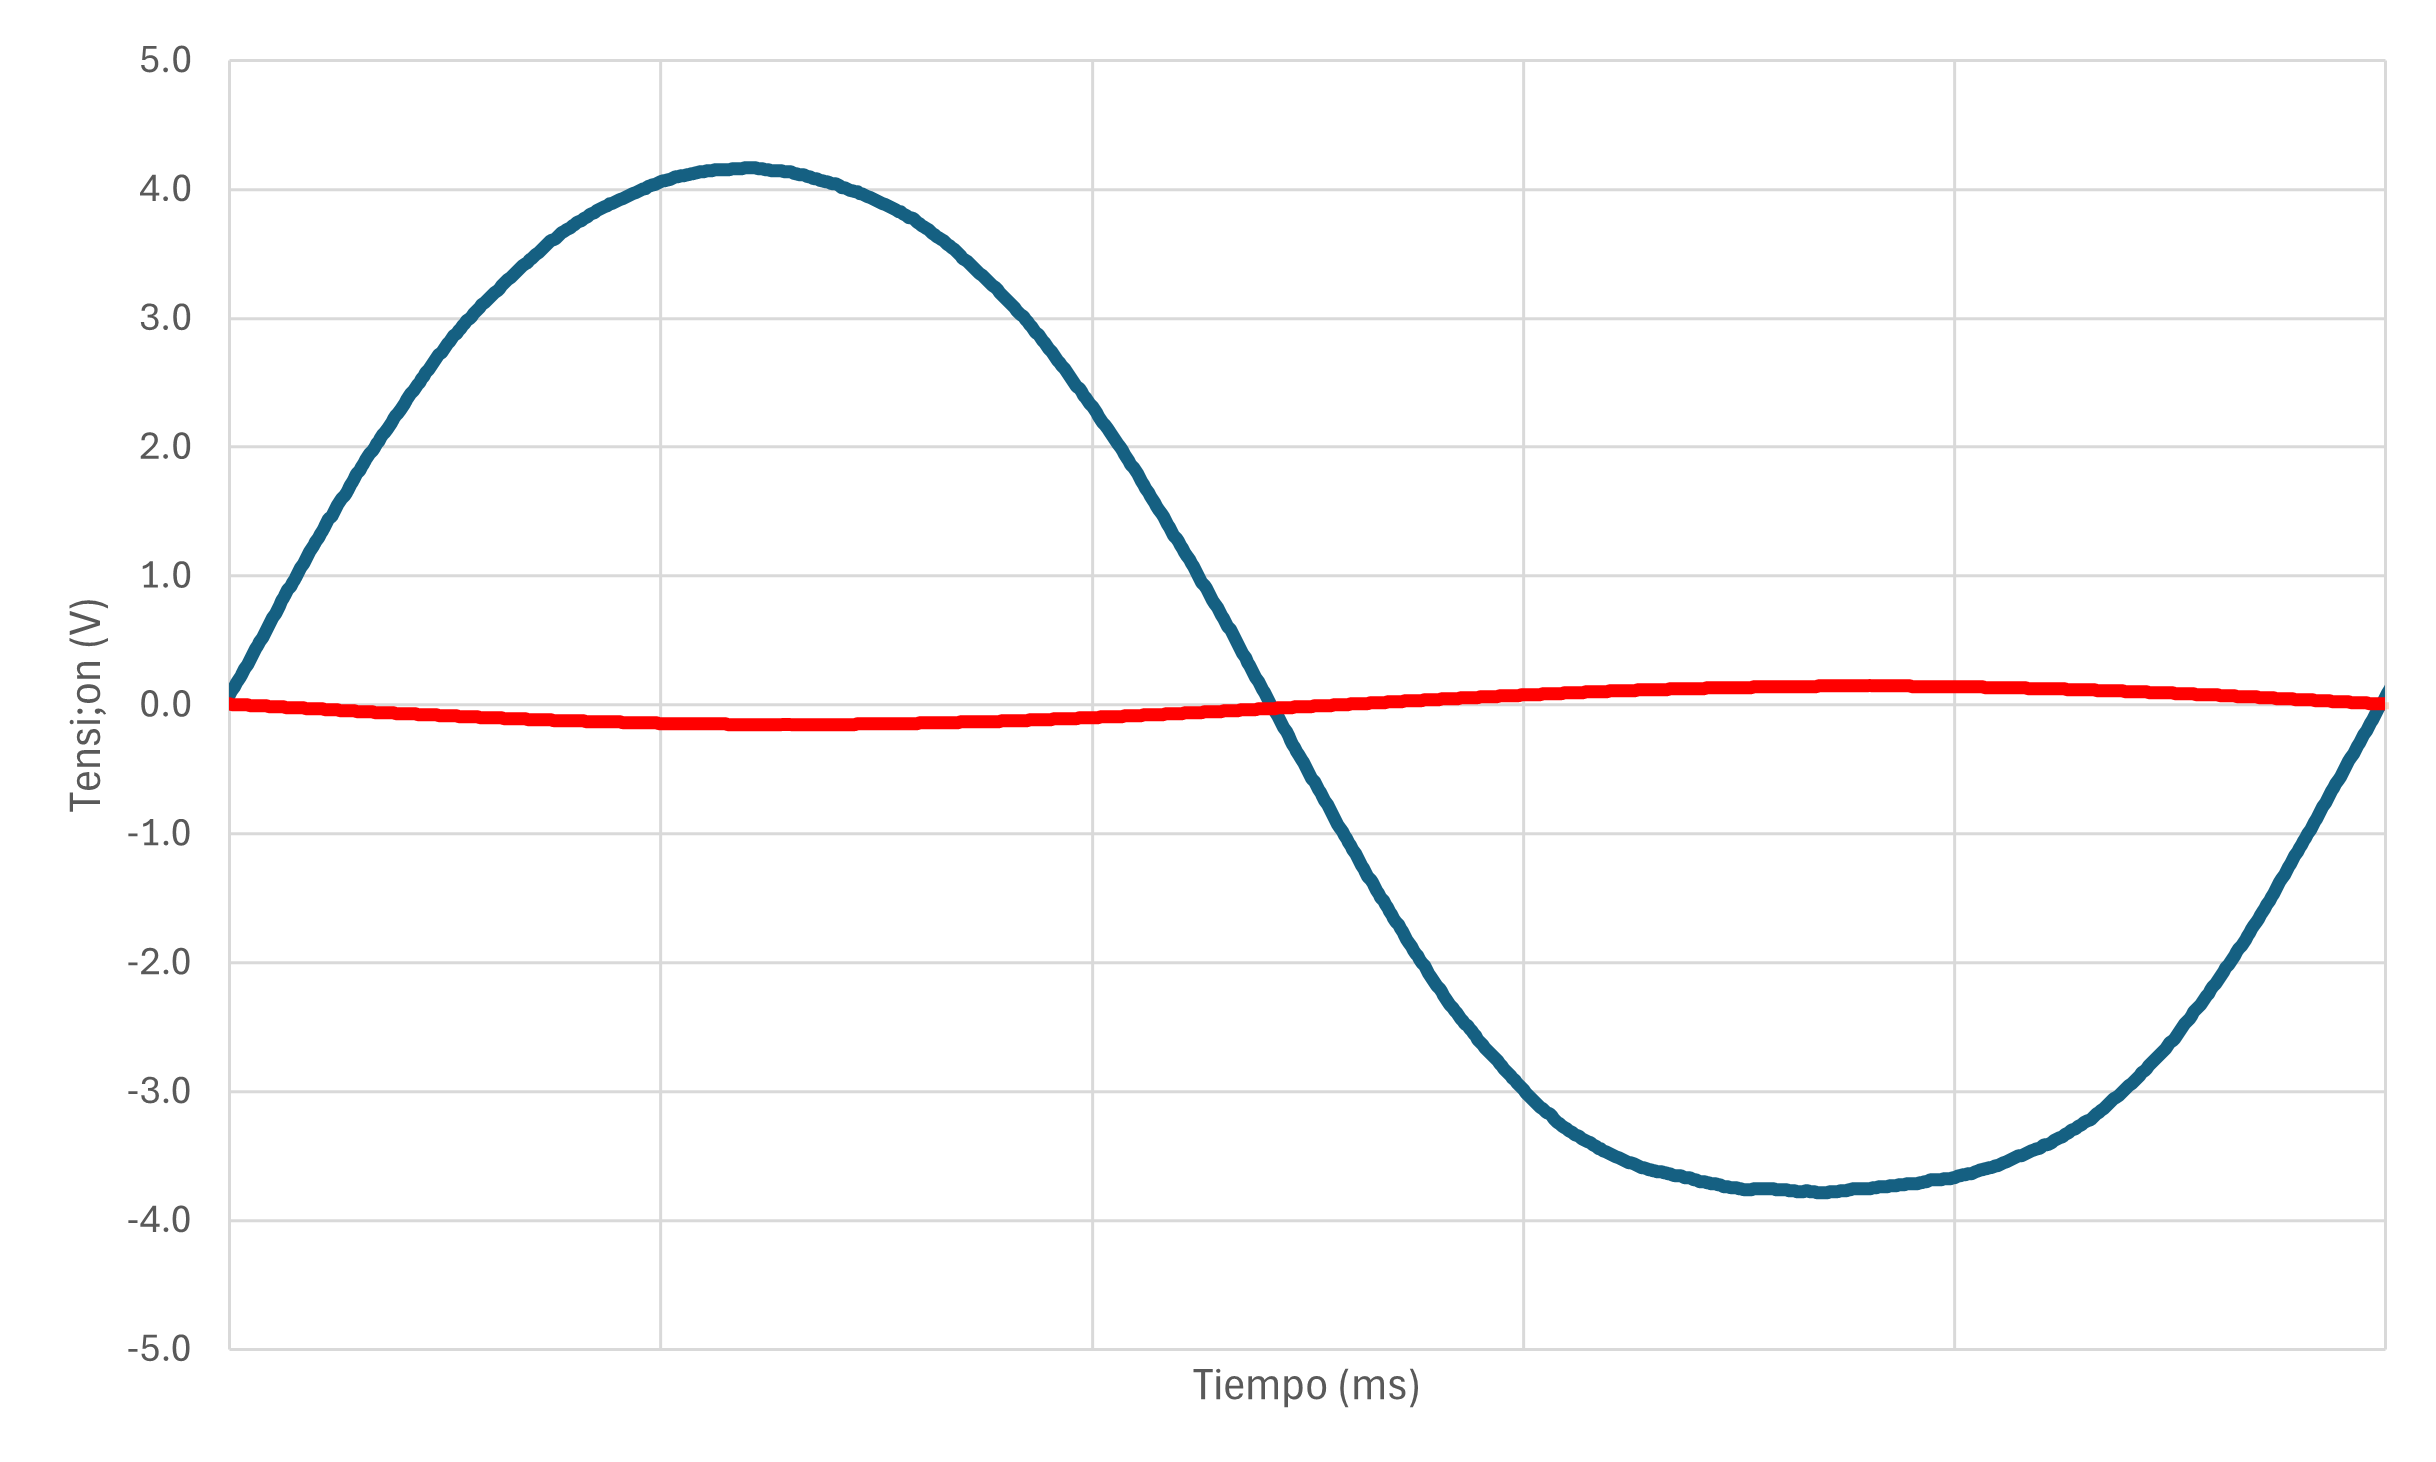
\includegraphics[width=3.4in]{C1111.png}
        \caption{$V_{sal}$ (en azul) y $V_{ent}$ (en rojo) obtenidos experimentalmente en el circuito 1 durante un periodo}
        \label{fig:SignalExperimental_02}
\end{figure}

\begin{figure}[H]
        \centering
        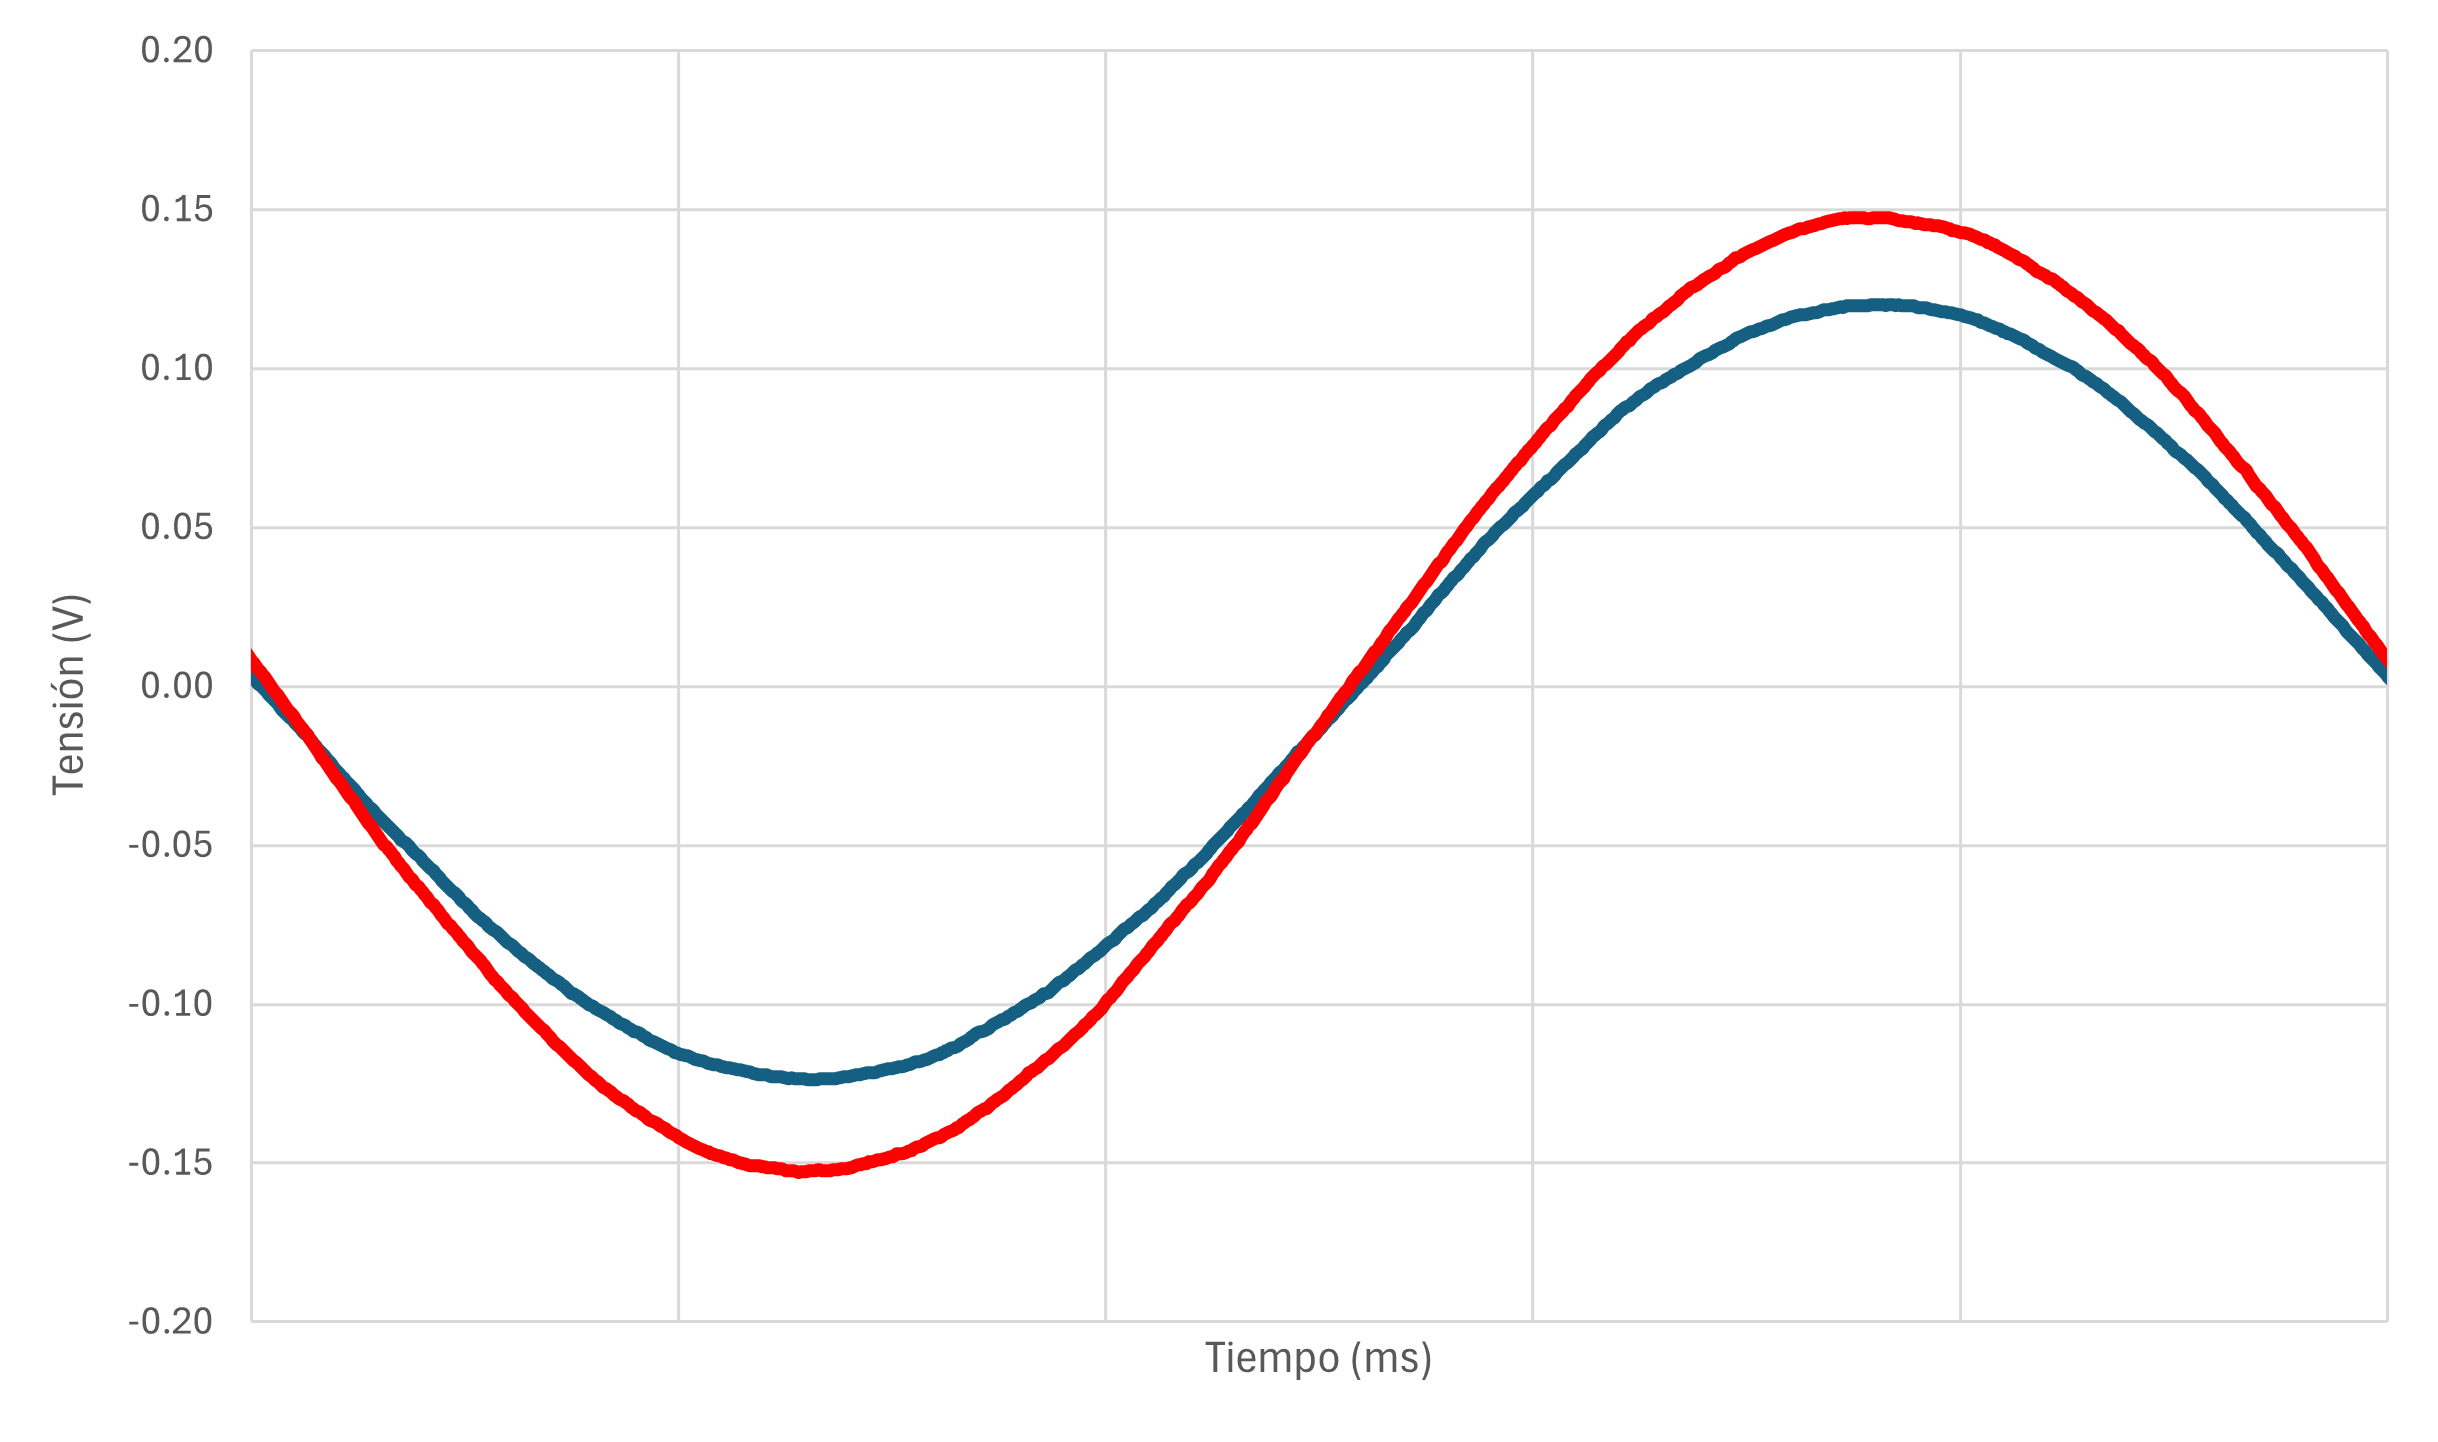
\includegraphics[width=3.4in]{C2222.png}
        \caption{$V_{sal}$ (en azul) y $V_{ent}$ (en rojo) obtenidos experimentalmente en el circuito 2 durante un periodo}
        \label{fig:SignalExperimental_03}
\end{figure}

\begin{figure}[H]
        \centering
        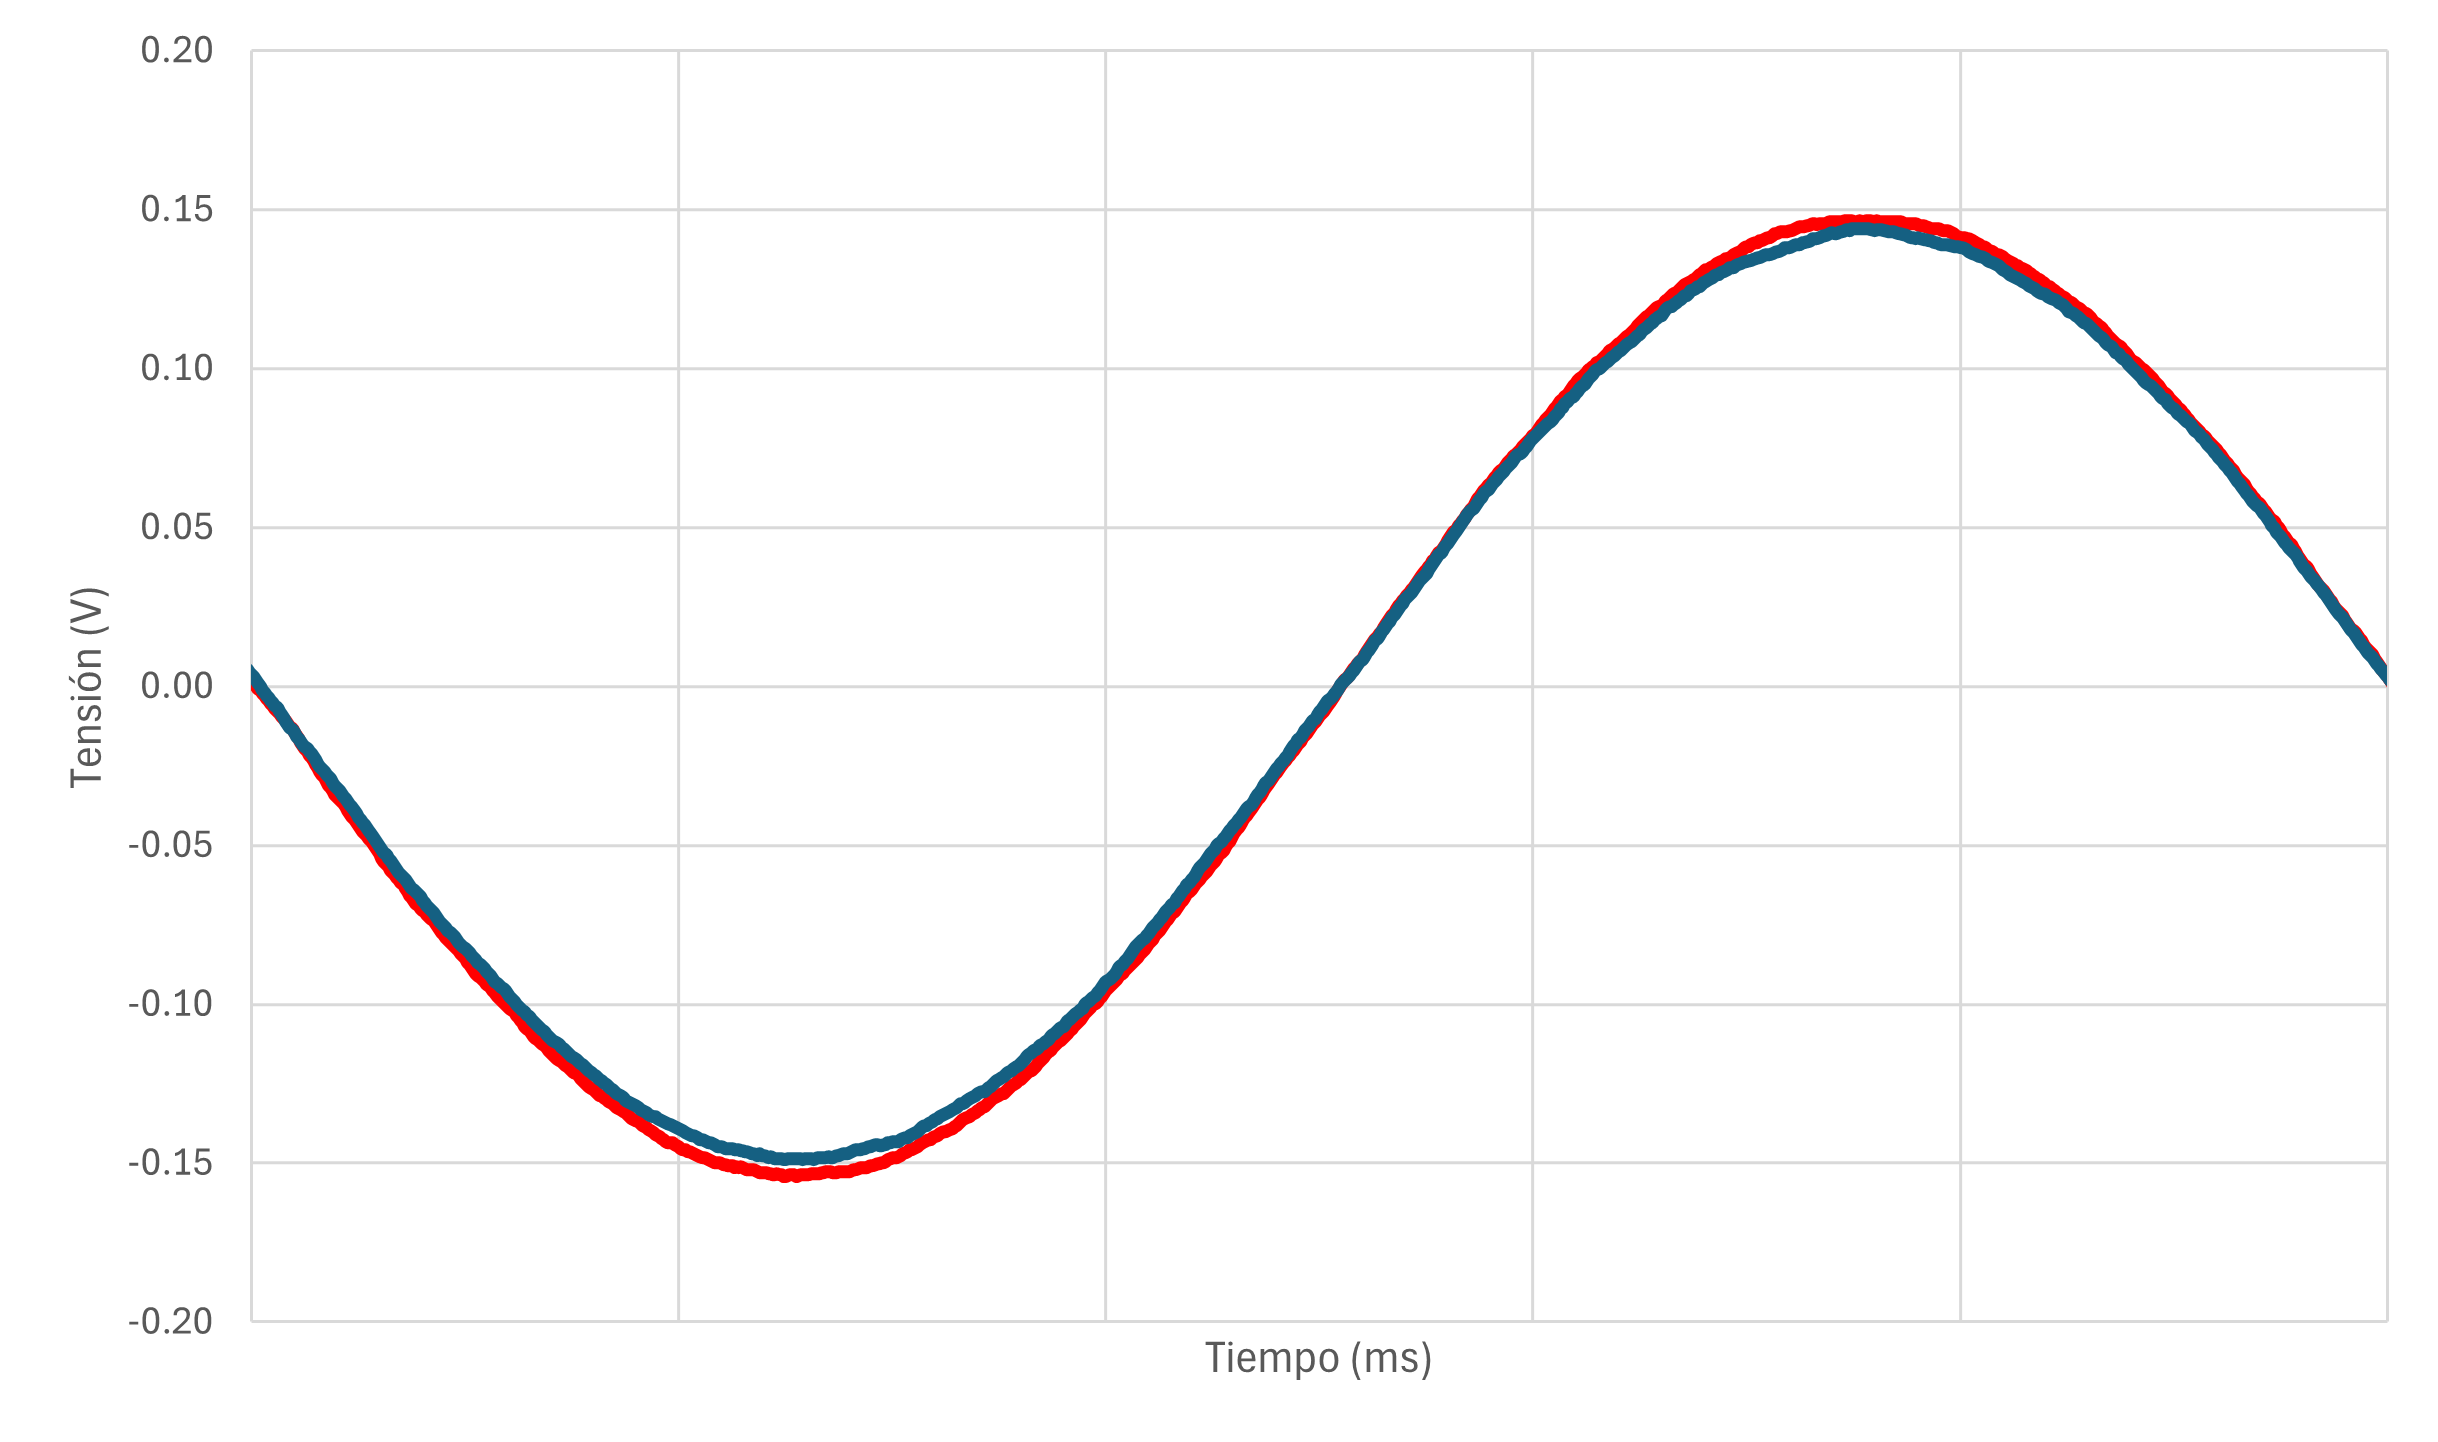
\includegraphics[width=3.4in]{2C2222.png}
        \caption{$V_{sal}$ (en azul) y $V_{ent}$ (en rojo) obtenidos experimentalmente en el circuito 3 durante un periodo}
        \label{fig:SignalExperimental_04}
\end{figure}

\begin{table}[H]
        \renewcommand{\arraystretch}{1.5}
        \caption{Mediciones del circuito 1}
        \centering
        \begin{tabular}{ >{\centering\arraybackslash}m{2.5cm} >{\centering\arraybackslash}m{2.5cm} >{\centering\arraybackslash}m{2.5cm} }
                \hline
            Parámetro & Valor teórico & Valor medido\\ 
            \hline
            $V_G$ & $6.763~52$ $\upmu\mathrm{V}$ & $209.6$ $\upmu\mathrm{V}$ \\ 
            $V_S$ & $71.312~86$ $\mathrm{mV}$ & $116.153$ $\mathrm{mV}$ \\
            $V_D$ & $6.340~58$ $\mathrm{V}$ & $4.052~65$ $\mathrm{V}$ \\
            $I_D$ & $1.273~44$ $\mathrm{mA}$ & $1.873~44$ $\mathrm{mA}$ \\
            $V_{ent}$ & $0.149~891$ $\mathrm{V}$ & $0.155$ $\mathrm{V}$ \\ 
            $V_{sal}$ & $4.635~36$ $\mathrm{V}$ & $3.9$ $\mathrm{V}$ \\
            $A_v$ & $30.2577$ & $25.16$ \\
            $Desfase$ & $-172.818~68^{\circ}$  & $-177.27^{\circ}$ \\
            \hline
        \end{tabular}
        \label{tabla6}
    \end{table}

\begin{table}[H]
        \renewcommand{\arraystretch}{1.5}
        \caption{Mediciones del circuito 2}
        \centering
        \begin{tabular}{ >{\centering\arraybackslash}m{2.5cm} >{\centering\arraybackslash}m{2.5cm} >{\centering\arraybackslash}m{2.5cm} }
                \hline
            Parámetro & Valor teórico & Valor medido\\ 
            \hline
            $V_G$ & $15.571~90$ $\upmu\mathrm{V}$ & $0.0018$ $\mathrm{V}$ \\
            $V_S$ & $209.402~04$ $\mathrm{mV}$ & $330.190$ $\mathrm{mV}$ \\
            $V_D$ & $15$ $\mathrm{V}$ & $15.0059$ $\mathrm{V}$ \\
            $I_D$ & $209.403~01$ $\upmu\mathrm{A}$ & $330.121$ $\upmu\mathrm{A}$ \\
            $V_{ent}$ & $0.149~949$ $\mathrm{V}$ & $0.157$ $\mathrm{V}$ \\ 
            $V_{sal}$ & $0.128~361$ $\mathrm{V}$ & $0.1265$ $\mathrm{V}$ \\
            $A_v$ & $0.856$ & $0.806$ \\
            $Desfase$ & $0.09^{\circ}$  & $1.19^{\circ}$ \\
            \hline
        \end{tabular}
        \label{tabla7}
    \end{table}

\begin{table}[H]
        \renewcommand{\arraystretch}{1.5}
        \caption{Mediciones del circuito 3}
        \centering
        \begin{tabular}{ >{\centering\arraybackslash}m{2.5cm} >{\centering\arraybackslash}m{2.5cm} >{\centering\arraybackslash}m{2.5cm} }
                \hline
            Parámetro & Valor teórico & Valor medido\\ 
            \hline
            $V_{G(Q1)}$ & $0$ $\mathrm{V}$ & $0.0018$ $\mathrm{V}$ \\ 
            $V_{S(Q1)}$ & $157.676~13$ $\mathrm{mV}$ & $160.81$ $\mathrm{mV}$ \\
            $V_{D(Q1)}$ & $15$ $\mathrm{V}$ & $15.0059$ $\mathrm{V}$ \\
            $V_{G(Q2)}$ & $-15.571~90$ $\mathrm{V}$ & $-15.0056$ $\mathrm{V}$ \\ 
            $V_{S(Q2)}$ & $-14.842~32$ $\mathrm{V}$ & $-14.7695$ $\mathrm{V}$ \\ 
            $V_{D(Q2)}$ & $0$ $\mathrm{V}$ & $0.0018$ $\mathrm{V}$ \\ 
            $I_D$ & $716.380$ $\upmu\mathrm{A}$ & $975.100$ $\upmu\mathrm{A}$ \\
            $V_{ent}$ & $0.15$ $\mathrm{V}$ & $0.157$ $\mathrm{V}$ \\ 
            $V_{sal}$ & $0.1448$ $\mathrm{V}$ & $0.151$ $\mathrm{V}$ \\
            $A_v$ & $0.965$ & $0.962$ \\
            $Desfase$ & $0^{\circ}$  & $0^{\circ}$ \\
            \hline
        \end{tabular}
        \label{tabla8}
    \end{table}

\subsection{Análisis de Resultados}
Los resultados obtenidos en el laboratorio fueron satisfactorios, lo que permite considerar la experiencia como provechosa. 
Entre los aspectos más destacados se encuentra el mayor entendimiento de la estructura general de cada uno de los circuitos utilizados, 
resultado de la interacción directa con componentes y dispositivos físicos. Esto resalta la importancia de prestar atención a las conexiones y a los 
métodos de medición para garantizar la recolección de datos de manera correcta y precisa.

Los datos y gráficas obtenidos reflejaron el comportamiento esperado y previamente estudiado en el entorno de simulación. 
Sin embargo, se observaron algunas variaciones en ciertas magnitudes del circuito (al momento de alterar ciertas conexiones por razones varias), 
lo que requirió ajustes en los parámetros de medición de los equipos. 
Para mejorar la interpretación de los resultados, es necesario considerar posibles alteraciones en las señales debidas a escalas de 
representación o interferencias de ruido.

\section{Conclusiones}
Se puede apreciar que las ondas de salida obtenidas durante el experimento siguieron la forma que se esperaba. A pesar de pequeñas diferencias
en cuanto a las amplitudes esperadas, el comportamiento general de la onda fue el calculado, por lo que el objetivo del experimento de construir circuitos recortadores
para entender el comportamiento de distintas ondas de salida fue cumplido exitosamente.

\appendices

\section{}
\vspace{-1.2cm}
\begin{IEEEbiographynophoto}{Matías A. Camacho Abarca}
        Estudiante del Instituto Tecnológico de Costa Rica en la carrerra de ingeniería en electrónica desde
        2023. Beneficiario de beca de excelencia académica por el Instituto Tecnológico de
        Costa Rica desde 2023. Como estudiante, sus
        intereses incluyen investigación y desarrollo.
        Correo electrónico: jeacamacho@estudiantec.cr
\end{IEEEbiographynophoto}
\vspace{-1.2cm}
\begin{IEEEbiographynophoto}{Juan P. Elizondo Espinoza}
        Oriundo de Pérez Zeledón. Realizó sus estudios de secundaria en el SNCCCR, sede UNA Región Brunca, y actualmente cursa la carrera de Ingeniería Electrónica en el Instituto Tecnológico de Costa Rica (TEC). 
        
        Anteriormente, fue estudiante de la Universidad de Costa Rica (UCR) durante el año 2022 y participó en programas de estudio en matemática en la Universidad Nacional (UNA) durante los años 2020 y 2021. 
        
        Cuenta con preparación y/o experiencia en áreas como:
        \begin{itemize}
            \item Arquitectura básica de redes, certificado por CISCO CCNA V7 (ITN), (2021).
            \item Principios de ciberseguridad, certificado por CISCO Systems, (2022).
            \item Programa de tutorías estudiantiles, Tecnológico de Costa Rica, (2024).
        \end{itemize}
        
        Correo: juelizondo@estudiantec.cr
\end{IEEEbiographynophoto}

\bibliographystyle{IEEEtran}
\bibliography{literatura}

\end{document}